\documentclass[../algebraIII_notes.tex]{subfiles}
\begin{document}
\section{Aula 15 - 02 de Junho, 2026}
\subsection{Motivações}
\begin{itemize}
	\item Mais exemplos de aplicação;
	\item Extensões Ciclotômicas.
\end{itemize}
\subsection{Extensões Ciclotômicas}
Antes do mais novo assunto, que vai ser usado para um exemplo futuro, vamos retomar o exemplo prévio:
\begin{example}[Mais Complicado]
	Desta vez, vamos considerar \(\mathbb{F} = \mathbb{Q}\) e \(f(x)=x^{3}-2\in \mathbb{F}[x]\); queremos \textbf{encontrar um corpo de decomposição} de \(f(x)\) sobre \(\mathbb{F}\), e, uma vez que tenhamos ele, procuraremos uma extensão normal finita, que será de Galois.
	Observe que, se fizermos \(f'(x)\), obtemos
	\[
		f'(x) = 3x^{2} \Rightarrow \mathrm{mdc}(f(x), f'(x))=1,
	\]
	tal que \(f(x)\) é separável. O próximo passo natural é \textbf{buscar as raízes de f}:
	\[
		\alpha_1 = \sqrt[3]{2}, \quad \alpha_2 = \sqrt[3]{2}\biggl(\frac{-1+\sqrt[]{-3}}{2}\biggr) \quad\&\quad \alpha_3 = \sqrt[3]{2}\biggl(\frac{-1-\sqrt[]{-3}}{2}\biggr),
	\]
	obtidas resolvendo o polinômio quadrático obtido ao fatorar \(x-\sqrt[3]{2}\)
	\[
		x^{3}-2 = (x-\sqrt[3]{2})(x^{2}+\sqrt[3]{2}x + \sqrt[3]{4}).
	\]
	Um corpo de decomposição de \(f(x)\) é, então, \(\mathbb{K} = \mathbb{Q}(\sqrt[3]{2}, \sqrt[]{-3})\)

	Tendo conhecimento do corpo de decomposição, precisamos \textbf{determinar o grau da extensão}, que pode ser feito escolhendo um caminho na torre (não contém todos os subcorpos possíveis!)
	\begin{center}
		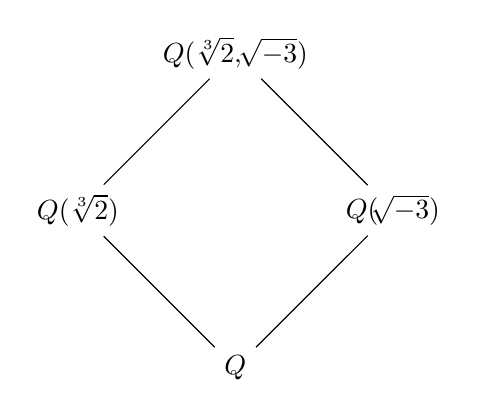
\begin{tikzpicture}[
				observed/.style = {rectangle, thick, text centered, draw, text width = 6em},
				latent/.style = {ellipse, thick, draw, text centered, text width = 6em},
				error/.style ={circle, thick, draw, text centered},
				confounding/.style = {rectangle, thick, text centered, draw, text width = 6em, minimum width = 5.5in},
				outcome/.style = {rectangle, thick, draw, text centered, minimum height = 3.5in, text width = 6em},
			]
			\node(TT) at (0,0){\(\mathbb{Q}(\sqrt[3]{2}, \sqrt[]{-3})\)};
			\node(TR) at (-2,-2){\(\mathbb{Q}(\sqrt[3]{2})\)};
			\node(CR) at (2,-2){\(\mathbb{Q}(\sqrt[]{-3})\)};
			\node(BB) at (0,-4){\(\mathbb{Q}\)};

			\draw[-](BB)--(CR);
			\draw[-](BB)--(TR);
			\draw[-](CR)--(TT);
			\draw[-](TR)--(TT);
		\end{tikzpicture}
	\end{center}
	Pela direita, o polinômio minimal é \(p(x) = x^{2}+3\), e, pela esquerda, é \(f(x)=x^{3}-2\); logo, pelo mesmo raciocínio de antes,
	\[
		[\mathbb{Q}(\sqrt[3]{2}, \sqrt[]{-3}):\mathbb{Q}]=[\mathbb{Q}(\sqrt[3]{2}):\mathbb{Q}(\sqrt[3]{2})][\mathbb{Q}(\sqrt[3]{2}):\mathbb{Q}]=3 \times 2 = 6,
	\]
	tal que
	\[
		\mathrm{ord}(\mathrm{Gal}(\mathbb{Q}(\sqrt[3]{2}, \sqrt[]{-3})/\mathbb{Q}))=6.
	\]

	Será que conseguimos \textbf{dar uma cara aos elementos do grupo de Galois}? Neste caso, queremos provar que \(\mathrm{Gal}(\mathbb{Q}(\sqrt[3]{2}, \sqrt[]{-3})/\mathbb{Q})\cong S_{3}\), e um argumento que podemos usar é mostrar que existe um isomorfismo:
	\begin{align*}
		\Lambda : & \mathrm{Gal}(\mathbb{Q}(\sqrt[3]{2}, \sqrt[]{-3})/\mathbb{Q})\rightarrow S_{3} \\
		          & \phi \longmapsto  \sigma_{\phi },
	\end{align*}
	onde
	\[
		\phi (\alpha_{i}) = \alpha_{\sigma_{\phi }(i)}
	\]
	é a ordenação/permutação das raízes por \(\sigma_{\phi }\), de modo que \(\Lambda(\varphi ) = \sigma_{\varphi }\).

	Temos que mostrar que este \(\Lambda \) é um homomorfismo injetor, pois isto dá o isomorfismo que queríamos. Com efeito, para ver que \(\Lambda \) é um homomorfismo de grupos, note que
	\[
		\Lambda (\varphi \psi ) = \sigma_{\varphi \psi },
	\]
	e
	\begin{align*}
		(\varphi \psi )(\alpha_{i}) = \varphi (\psi (\alpha_{i})) & = \varphi(\alpha_{\sigma_{\psi }(i)})           \\
		                                                          & = \alpha_{\sigma_{\varphi }(\sigma_{\psi }(i))} \\
		                                                          & = \alpha_{\sigma_{\psi }(\sigma_{\varphi }(i))} \\
		                                                          & =(\psi \varphi )(\alpha_{i}).
	\end{align*}
	Logo, para todos \(\varphi , \psi\),
	\[
		\Lambda (\varphi \psi ) = \Lambda (\psi \varphi ).
	\]
	Ademais,
	\[
		\Lambda (\mathrm{id}) = \sigma_{\mathrm{id}} = \mathrm{id}_{S_{3}},
	\]
	restando apenas mostrar a injetividade. De fato,
	\[
		\mathrm{ker}(\Lambda ) = \{\varphi \in \mathrm{Gal}(\mathbb{K}/\mathbb{F}):\; \Lambda (\varphi ) = \mathrm{id}_{S_{3}}\},
	\]
	mas
	\[
		\Lambda (\varphi ) = \sigma_{\varphi } = \mathrm{id}\in S_{3}\Longleftrightarrow \sigma_{\varphi }(i) = i, \quad i=1, 2, 3.
	\]
	Assim, se \(\varphi \) for um elemento no núcleo de \(\Lambda \), vale
	\[
		\varphi (\alpha_{i})=\alpha_{\sigma_{\varphi }(i)} = \alpha_{i} \Rightarrow \varphi\in \mathrm{ker}\Lambda \Longleftrightarrow \varphi(\alpha_{i})=\alpha_{i},
	\]
	ou seja, \(\mathrm{ker}(\Lambda ) = \{\mathrm{id}\}\). Como os dois grupos têm a mesma ordem e existe um homomorfismo injetor entre eles, vale \(\Lambda \) é um isomorfismo entre os grupos.

	Agora que temos essa informação, podemos tentar analisar um pouco essa extensão pelo ponto de vista do \hyperlink{fundamental_galois}{\textit{teorema fundamental}}, considerando todos os subgrupos de \(S_{3}\) para obter as subextensões. Como essa correspondência é injetora, encontrar todos os subgrupo leva a todas as subextensões!
	Vamos procurar os subgrupos de \(S_{3}\): primeiramente, \(S_{3} \) é um grupo de ordem 3, tal que seus subgrupos têm ou ordem 3, ou ordem 2, e com a notação de ciclos, caracteriza-se \(S_{3}\) pelas permutações:
	\[
		S_{3} = \{\mathrm{id}, \underbrace{(12), (13), (23)}_{\text{ordem 2}}, \underbrace{(123), (132)}_{\text{ordem 3}}\}.
	\]
	Logo, temos 3 elementos de ordem 2 que gerarão 3 subgrupos de ordem 2, e 2 elementos de ordem 3 que gerarão 2 subgrupos de ordem 3; apesar dos elementos serem distintos, \((123)^{2}=(132)\), tal que eles geram o mesmo subgrupo:
	\[
		\langle (123) \rangle = \langle (132) \rangle = A_{3},
	\]
	que é o grupo alternado de 3 elementos. Cada um dos subgrupos de ordem 2 gerados pelos elementos não é normal (exercício), e a situação aqui é a seguinte:
	\begin{center}
		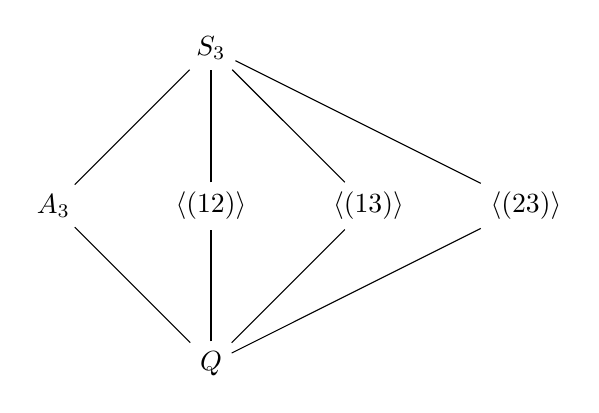
\begin{tikzpicture}[
				observed/.style = {rectangle, thick, text centered, draw, text width = 6em},
				latent/.style = {ellipse, thick, draw, text centered, text width = 6em},
				error/.style ={circle, thick, draw, text centered},
				confounding/.style = {rectangle, thick, text centered, draw, text width = 6em, minimum width = 5.5in},
				outcome/.style = {rectangle, thick, draw, text centered, minimum height = 3.5in, text width = 6em},
			]
			\node(TT) at (0,0){\(S_3\)};
			\node(TR) at (-2,-2){\(A_3\)};
			\node(CL) at (0,-2){\(\langle (12) \rangle\)};
			\node(CR) at (2,-2){\(\langle (13) \rangle\)};
			\node(CRR) at (4,-2){\(\langle (23) \rangle\)};
			\node(BB) at (0,-4){\(\mathbb{Q}\)};

			\draw[-](BB)--(CR);
			\draw[-](BB)--(CRR);
			\draw[-](BB)--(TR);
			\draw[-](BB)--(CL);
			\draw[-](CL)--(TT);
			\draw[-](CR)--(TT);
			\draw[-](CRR)--(TT);
			\draw[-](TR)--(TT);
		\end{tikzpicture}
	\end{center}
	A partir disso, as subextensões de \(\mathbb{K}/\mathbb{F}\) serão o \(\mathrm{Inv}(\cdot )\) para cada um dos subgrupos:
	\begin{align*}
		 & \mathrm{Inv}(A_3) = \mathbb{Q}(\omega )                                 \\
		 & \mathrm{Inv}(\langle (12) \rangle) = \mathbb{Q}(\omega^{2}\sqrt[3]{2} ) \\
		 & \mathrm{Inv}(\langle (13) \rangle) = \mathbb{Q}(\omega\sqrt[3]{2} )     \\
		 & \mathrm{Inv}(\langle (23) \rangle) = \mathbb{Q}(\sqrt[3]{2}).
	\end{align*}

	Sendo \(A_3\) um subgrupo normal de \(S_3\), a extensão \(\mathrm{Inv}(A_3)/\mathbb{Q}\) é normal; por outro lado, \(\mathbb{Q}(\sqrt[3]{2})/\mathbb{Q}\) não é normal!
	No entanto, sendo \(\mathrm{Inv}(A_3)= \mathbb{Q}(\omega)\), a extensão \(\mathbb{Q}(\omega )/\mathbb{Q}\) é normal, com polinômio minimal de \(\omega \) sobre \(\mathbb{Q}\) dado por
	\[
		p(x) = x^{2}+x+1 = (x-\omega )(x-\overline{\omega }),
	\]
	tal que \(\mathbb{Q}(\omega)\) é um corpo de decomposição de \(p(x)\).
\end{example}
\begin{exr}
	Mostre as relações das subextensões restantes, e que cada um dos subcorpos associados aos grupos gerados é normal.
\end{exr}

Vamos iniciar este assunto considerando o polinômio \(f(x)=x^{n}-1\in \mathbb{F}[x]\), com \(\mathbb{F}\) podendo ser tanto um corpo com característica 0, quanto característica p (por enquanto).
\begin{def*}
	As soluções de \(f(X) = 0\) são chamadas \textbf{raízes n-ésimas da unidade}. \(\square\)
\end{def*}
\begin{example}[Brincando com Características de Corpos]
	Vamos supor que\linebreak\(\mathrm{char}(\mathbb{F}) = p\), p primo; então, \(\alpha \) é uma raiz n-ésima de 1 se, e somente se, \(\alpha =1\), pois
	\[
		x^{n}-1=0 \Longleftrightarrow (x-1)^{n} = 0.
	\]

	Porém, se \(\mathbb{F} = \mathbb{Q}\), então \(\alpha \) é uma raiz n-ésimas da identidade se, e somente se, existe \(0\leq k\leq n-1\) tal que
	\[
		\alpha_{k}= e^{\frac{2\pi i}{n}k}.
	\]
	Claramente, há uma pequena diferença entre os casos, e há uma certa ciclicidade das raízes, pois o caso \(k=n\) seria equivalente a um múltiplo par de \(2\pi \), que é o mesmo que o caso \(0\) (similarmente, todos os outros casos se repetem), e por isso restringimos apenas aos números entre 0 e n-1: evita redundância.
\end{example}
\begin{lemma*}
	Seja \(\mathcal{M}_{n}\) o conjunto das raízes n-ésimas da unidade; então, \(\mathcal{M}_{n}\) é um grupo abeliano de ordem n.
\end{lemma*}
Seria interessante enocntrarmos os elemnetos que geram este grupo, pois permitiria determinarmos quais são cíclicos. Doravante, suponhamos que \(\mathbb{F} = \mathbb{Q}\), e mantenhamos a notação
\[
	\mathcal{M}_{n} = \biggl\{\alpha_{k} \coloneqq e^{\biggl(\frac{2\pi i}{n}k\biggr)}:\; 0\leq k\leq n-1\biggr\}.
\]
Afirmamos que \(\mathcal{M}_{n}\) é um grupo cíclico de ordem n se, e somente se, k e n são coprimos, ou seja, \(\mathrm{mdc}(k, n) = 1\).

Em \(\mathcal{M}_{n}\), temos \(\varphi (n)\) geradores, onde \(\varphi \) é a chamada \textbf{função Totiente de Euler}, que conta o número de elementos coprimos de k:
\[
	\varphi (k) = \# \{\ell : 1\leq \ell < k,\; (\ell , k)=1\}
\]
\begin{def*}
	Uma raiz n-ésima da unidade, \(\alpha \), é chamada \textbf{primitiva} se ela é uma geradora de \(\mathcal{M}_{n}.\; \square\)
\end{def*}
\begin{example}
	\begin{itemize}
		\item[n=1:] para \(n=1\), a raiz \(\alpha =1\) é primitiva; o polinômio correspondente é \(f(x) = x-1\);
		\item[n=2:] para \(n=2\), a raiz \(\alpha =-1\) é a única primitiva; o polinômio correspondente é \(f(x) = x^{2}-1\) (note que \(1 = -1 \times -1\), portanto \(-1\) gera a outra raiz da unidade);
		\item[n=3:] para \(n=3\), as raízes primitivas são \(\displaystyle \alpha_1 =\mathrm{exp}\biggl(\frac{2\pi i}{3}\biggr)\) e \(\displaystyle \alpha_2 = \mathrm{exp}\biggl(\frac{4\pi i}{3}\biggr)\); o polinômio correspondente é \(f(x) = x^{3}-1\), e o grupo cíclico é
		      \[
			      \mathcal{M}_{3} = \biggl\{\mathrm{exp}\biggl(\frac{2\pi i}{3}k\biggr):\; 0\leq k \leq 2\biggr\} = \biggl\{1, \mathrm{exp}\biggl(\frac{2\pi i}{3}\biggr), \mathrm{exp}\biggl(\frac{4\pi i}{3}\biggr)\biggr\};
		      \];
		\item[n=4:] para \(n=4\), as raízes primitivas são \(\displaystyle \alpha_1 =\mathrm{exp}\biggl(\frac{\pi i}{2}\biggr)=i\) e \(\displaystyle \alpha_2 = \mathrm{exp}\biggl(\frac{3\pi i}{2}\biggr)=-i\); o polinômio correspondente é \(f(x) = x^{4}-1\), e o grupo cíclico é
		      \[
			      \mathcal{M}_{4} = \biggl\{\mathrm{exp}\biggl(\frac{\pi i}{2}k\biggr):\; 0\leq k \leq 3\biggr\} = \{1, i, -i, -1\}.
		      \];
	\end{itemize}
\end{example}
\begin{def*}
	O \textbf{n-ésimo polinômio ciclotômico} é o polinômio
	\[
		C_{n}(x) = \prod\limits_{(k, n)=1}^{}(x-\alpha_{k}),\; \alpha_{k}\in \mathcal{M}_{n}.
	\]
\end{def*}
Em outras palavras, o n-ésimo polinômio ciclotômico é o produto da incógnita subtraída das raízes primitivas da unidade.
\begin{example}
	Vamos ver alguns dos polinômios, para alguns dos n's:
	\begin{align*}
		 & \tikz[baseline=-0.5ex]\draw[black, fill=black, radius=1.5pt](0, 0)circle;\; C_{1}(x) = x-1                                                                                                          \\
		 & \tikz[baseline=-0.5ex]\draw[black, fill=black, radius=1.5pt](0, 0)circle;\; C_{2}(x) = (x-(-1))=x+1                                                                                                 \\
		 & \tikz[baseline=-0.5ex]\draw[black, fill=black, radius=1.5pt](0, 0)circle;\; C_{3}(x) = \biggl(x-e^{\bigl(\frac{2\pi i}{3}\bigr)}\biggr)\biggl(x-e^{\bigl(\frac{4\pi i}{3}\bigr)}\biggr) = x^{2}-x+1 \\
		 & \tikz[baseline=-0.5ex]\draw[black, fill=black, radius=1.5pt](0, 0)circle;\; C_{4}(x) = (x-i)(x+i)
	\end{align*}
\end{example}
\begin{lemma*}
	Seja \(n\geq 1\); vale a relação
	\[
		x^{n}-1 = \prod\limits_{d | n}^{}C_{d}(x).
	\]
\end{lemma*}
\begin{proof*}
	\textbf{A prova é deixada como exercício}. Complete os seguintes passos:
	\begin{itemize}
		\item[1)] Mostre que \(C_{d}(x)\) divide \(x^{d}-1\);
		\item[2)] Se d divide n, então \((x^{d}-1)\) divide \((x^{n}-1)\).
	\end{itemize}
	Com isto, 1 e 2 combinados darão
	\[
		\biggl(\prod\limits_{d|n}^{}C_{d}(x)\biggr) | x^{n}-1,
	\]
	e demonstrar o lema consistirá em exibir que o produto dos polinômios ciclotômicos podem ser fatorados por \(x^{n}-1\), i.e.,
	\[
		(x^{n}-1)| \prod\limits_{d|n}^{}C_d(x).
	\]
	Daí, é suficiente provar que, para todo k entre 1 e n-1, existe d dividindo n tal que \(C_{d}(\alpha_{k}) = 0.\) \qedsymbol
\end{proof*}
Uma coisa mais interessante, mas mais complexa de provar e que fica mais como um comentário, é que dá pra fazer o caminho inverso; para isso, utiliza-se a \textbf{função de Möbius}:
\[
	\mu (n)  = \left\{\begin{array}{ll}
		1,        & \quad n=1                                                 \\
		(-1)^{k}, & \quad n = p_1 \dotsc p_k,\; p_{k}\text{ primos distintos} \\
		0,        & \quad \exists x^{2}:\; x^{2}| n.
	\end{array}\right..
\]
Com isso,
\[
	\boxed{C_{n}(x) = \prod\limits_{d | n}^{}\biggl(x^{\frac{n}{d}}-1\biggr)^{\mu (d)}}
\]

Utilizando o lema, podemos demonstrar que
\begin{prop*}
	Para todos naturais n, o polinômio ciclotômico \textbf{sempre terá coeficientes inteiros}:
	\[
		C_{n}(x)\in \mathbb{Z}[x].
	\]
\end{prop*}
\begin{proof*}
	A prova segue por indução em n, sendo o caso base já mostrado no exemplo.
	Agora, assumindo que, para todo \(m < n\), temos \(C_{m}(x)\in \mathbb{Z}[x]\), então
	\[
		g(x)\coloneqq \prod\limits_{(d | n, d < n)}^{} C_{d}(x)\in \mathbb{Z}[x].
	\]
	Daí, podemos dividir \(x^{n}-1\) com o \hyperlink{euclides_algorithm}{\textit{algoritmo de Euclides}}
	\begin{align*}
		                   & x^{n}-1 = g(x)q(x) + r(x), \quad 0 \leq \deg{(r(x))} < \deg{(g(x))} \\
		\text{Pelo lema, } & x^{n}-1 = C_{n}(x)g(x)                                              \\
		\Rightarrow        & g(x)q(x) + r(x) = C_{n}(x)g(x)                                      \\
		\Rightarrow        & r(x) = (C_{n}(x)-q(x))g(x).
	\end{align*}
	Esta identidade não é absurda se, e somente se, \(r\equiv 0\), então concluímos que \(r(x) = 0\); em particular, \(q(x)=C_{n}(x)\) e \(q(x)\in \mathbb{Z}[x]\). \qedsymbol
\end{proof*}

Para introduzir as \textit{extensões ciclotômicas}, usaremos os polinômios ciclotômicos para gerá-las, e será um corpo se, e somente se, eles forem irredutíveis.
\begin{theorem*}
	Para todo natural n, \(C_{n}(x)\) é irredutível sobre \(\mathbb{Q}\).
\end{theorem*}
\begin{proof*}
	A estratégia de prova será por contradição: assumindo a redutibilidade de \(C_{n}(x)\), ou seja, que
	\[
		C_{n}(x) = h(x)k(x), \quad h(x), k(x)\in \mathbb{Zj[x]},
	\]
	assumindo ambos mônicos e que h é irredutível, vamos mostrar que, para cada z complexo tal que z é raiz de h, então \(h(z^{r}) = 0\) para todo r coprimo de n, e isso finalizará a demonstração.

	Com efeito, a propriedade mencionada é consequência de que, se \(h(z) = 0\), então \(h(z^{p}) = 0\) para todo p primo que não divide n, e vamos mostrar isso, pois dela, basta considerar r tal que \((r, n)=1\) e decompor
	\[
		r = p_1 p_2 \dotsc p_s,
	\]
	possivelmente com multiplicidade maior que 1; daí, como \((r, n) = 1\), necessariamente temos \(p_{i}\) não podendo dividir r para todo i; então, se \(h(z) = 0\), teremos
	\[
		h(z^{p_1}) = 0 \Rightarrow h((z^{p_1})^{p_2}) = 0 \Rightarrow \dotsc \Rightarrow h((z^{p_1 \dotsc p_{s-1}})^{p_s}) = 0 \Longleftrightarrow h(z^{r}) = 0.
	\]

	Sem mais delongas, suponha que \(h(z) = 0\) e seja \(p\) um primo que não divide n, tais que \(h(z^{p}) \neq 0\); então, necessariamente \(k(z^{p})=0\), e z é necessariamente uma raiz de \(k(x^{p})\).
	Daí, sendo \(h(x)\) irredutível e z uma raiz comum entre \(h(x)\) e \(k(x^{p})\), podemos concluir que \(h(x)\) divide \(k(x^{p})\):
	\[
		k(x^{p}) = h(x)\ell (x), \quad \ell (x)\in \mathbb{Z}[x].
	\]

	Então, por esta identidade, junto à relação abaixo (derivada do lema)
	\[
		x^{n}-1 = h(x)k(x)\underbrace{\prod\limits_{(d|n, d<n)}^{}C_{d}(x)}_{\coloneqq g(x)}.
	\]
	Por outro lado, se \(f(x) = a_{0}+ a_1 x + \dotsc + a_{n}x^{n}\) é um polinômio em \(\mathbb{Z}[x]\) e p é primo, então podemos definir
	\[
		\overline{f}(x) = \overline{a}_{0} + \overline{a}_1x + \dotsc  + \overline{a}_{n}x^{n}\in \mathbb{Z}_{p}[x], \quad \overline{a}_{i} = a_{i}\;\mathrm{mod}\;p;
	\]
	além disso, se \(\overline{f}(x)\in \mathbb{Z}_{p}[x]\), então
	\[
		\overline{f}(x)^{p} = \overline{f}(x^{p}),
	\]
	pois, para todo \(b_{i}\in A\) quando A é um anel de característica p,
	\[
		(b_1 + \dotsc  + b_{k})^{p} = b_1^{p} + (b_2 + \dotsc +b_{k})^{p} = b_1^{p}+\dotsc +b_{k}^{p},
	\]
	e ganhamos
	\begin{align*}
		(\overline{f}(x))^{p} & = (\overline{a}_{0} + \overline{a}_1x + \dotsc  + \overline{a}_{n}x^{n})^{p}            \\
		                      & = \overline{a}_{0}^{p} + \overline{a}_1^{p}x^{p} + \dotsc  + \overline{a}_{n}^{p}x^{np} \\
		                      & = \overline{f}(x^{p}).
	\end{align*}

	Para usar isso, temos
	\[
		x^{n}-\overline{1} =\overline{h}(x)\overline{k}(x)\overline{g}(x) \quad\&\quad \overline{k}(x^{p}) = \overline{h}(x)\overline{\ell }(x)\in \mathbb{Z}_{p}[x];
	\]
	logo,
	\[
		\overline{k}(x)^{p} = \overline{h}(x)\overline{\ell }(x)\in \mathbb{Z}_{p}[x].
	\]
	Disto, junto ao exercício abaixo, é preciso que \(x^{n}-\overline{1}\) possua raízes múltiplas (pois p foi escolhido tal que p não divide n), mas isto é uma contradição, porque
	\[
		\biggl(x^{n}-\overline{1}, \frac{\mathrm{d}}{\mathrm{d}x}(x^{n}-\overline{1})\biggr) = 1.
	\]
	Portanto, finalizamos a demonstração, pois mostramos que \(z^{p}\) é uma raiz de h para todo p que não divide n, e por isso \(C_{d}(x)\) é um divisor de h. \qedsymbol
\end{proof*}
\begin{exr}
	Mostre que \((\overline{h}(x), \overline{k}(x))\neq 1\).
\end{exr}
Com este teorema, ganhamos o corpo \(\mathbb{Q}[x]/\langle C_{n}(x) \rangle\), chamado \textbf{n-ésimo corpo ciclotômico}, denotado (talvez mude) por \(\mathbb{Q}(z_{n})\).
Pelo caso geral, vamos considerar a seguir o caso particular de n primo (que é muito mais simples) com o \textit{\hypertarget{eisenstein_criterion}{critério de Eisenstein}}:
\begin{prop*}[Critério de Eisenstein]
	Para um polinômio com coeficientes inteiros de grau n qualquer,
	\[
		p(x) = a_{n}x^{n} + \dotsc + a_1x + a_{0},
	\]
	ele será irredutível sobre os números racionais se existir um número primo p tal que:
	\begin{itemize}
		\item[i)] p divide cada \(a_{i}\) para \(i\neq n\);
		\item[ii)] p \textit{não divide} \(a_{n}\); e
		\item[iii)] \(p^{2}\) \textit{não divide} \(a_{0}\).
	\end{itemize}
\end{prop*}
\end{document}
